% !TEX root = main.tex
% !TEX program = pdflatex
\documentclass[aspectratio=169,10pt]{beamer}

\usetheme{Bruno}

\usepackage[T1]{fontenc}
\usepackage[utf8]{inputenc}
\usepackage[brazil]{babel}
\usepackage{graphicx}
\usepackage{booktabs}
\usepackage{tabularx}
\usepackage{array}
\usepackage{tikz}
\usetikzlibrary{arrows.meta,positioning,shapes.geometric}
\usepackage[most]{tcolorbox}
\usepackage{listings}
\usepackage{microtype}
\usepackage{ragged2e}

\graphicspath{{../images/figures/}{../images/mermaid/outputs/}}

\definecolor{collectorInk}{HTML}{12302F}
\definecolor{collectorTeal}{HTML}{1F8A70}
\definecolor{collectorMint}{HTML}{EAF7F1}
\definecolor{collectorCoral}{HTML}{D94F30}
\definecolor{collectorGold}{HTML}{F2B84B}
\definecolor{collectorGray}{HTML}{F3F6F4}
\definecolor{collectorLine}{HTML}{C9D8D2}

\setbeamercolor{normal text}{fg=collectorInk}
\setbeamercolor{structure}{fg=collectorTeal}
\setbeamercolor{frametitle}{fg=collectorInk}
\setbeamercolor{footline}{bg=collectorMint,fg=collectorInk}
\setbeamercolor{block title}{bg=collectorInk,fg=white}
\setbeamercolor{block body}{bg=collectorGray,fg=collectorInk}
\setbeamercolor{separator}{fg=collectorCoral,bg=collectorCoral}
\setbeamerfont{frametitle}{size=\Large,series=\bfseries}
\setbeamerfont{framesubtitle}{size=\small,shape=\normalfont}
\setbeamersize{text margin left=8mm,text margin right=8mm}

\newcolumntype{Y}{>{\RaggedRight\arraybackslash}X}
\newcolumntype{L}[1]{>{\RaggedRight\arraybackslash}p{#1}}

\newcommand{\collectorFlutter}{\texttt{collector\_flutter}}
\newcommand{\devtools}{\textit{Flutter DevTools}}
\newcommand{\jank}{\textit{jank}}
\newcommand{\rebuild}{\textit{rebuild}}
\newcommand{\rebuilds}{\textit{rebuilds}}
\newcommand{\overhead}{\textit{overhead}}
\newcommand{\chaptertag}[1]{\textcolor{collectorCoral}{\footnotesize\bfseries #1}\par\vspace{1mm}}
\newcommand{\smallref}[1]{\textcolor{collectorTeal}{\scriptsize #1}}

\tcbset{
  enhanced,
  boxrule=0.55pt,
  arc=1.5mm,
  left=1.5mm,
  right=1.5mm,
  top=1.1mm,
  bottom=1.1mm,
  colframe=collectorLine,
  colback=collectorGray,
  coltitle=collectorInk,
  fonttitle=\bfseries,
  before skip=1mm,
  after skip=1mm
}

\newtcolorbox{infobox}[2][]{
  title={#2},
  colback=collectorGray,
  colframe=collectorLine,
  #1
}

\newtcolorbox{accentbox}[2][]{
  title={#2},
  colback=collectorMint,
  colframe=collectorTeal,
  #1
}

\newcommand{\metric}[3]{%
  \begin{tcolorbox}[width=#1,colback=white,colframe=#2,boxrule=0.8pt]
    {\Large\bfseries\textcolor{#2}{#3}}
  \end{tcolorbox}
}

\lstdefinestyle{dart}{
  basicstyle=\ttfamily\scriptsize,
  keywordstyle=\bfseries\color{collectorTeal},
  commentstyle=\itshape\color{collectorInk!60},
  stringstyle=\color{collectorCoral},
  showstringspaces=false,
  breaklines=true,
  frame=single,
  framerule=0.4pt,
  rulecolor=\color{collectorLine},
  backgroundcolor=\color{collectorGray},
  columns=fullflexible
}

\IfFileExists{../images/figures/background.jpg}{\background{../images/figures/background.jpg}}{}

\title[Monitoramento Flutter]{Monitoramento e otimização de recursos em aplicativos Flutter}
\author[B. V. Frade]{Beatriz Vocurca Frade}
\institute{Universidade Federal de Minas Gerais\\Engenharia de Sistemas\\Orientador: Prof. Ramon Lacerda Marques}
\date{2026}

\begin{document}

\maketitle

\begin{frame}{Roteiro da defesa}
\chaptertag{20 minutos}
\begin{columns}[T,onlytextwidth]
  \column{0.33\textwidth}
  \begin{accentbox}{1. Problema}
    Contexto Flutter, motivação e pergunta de pesquisa.
  \end{accentbox}
  \begin{infobox}{2. Base}
    Literatura, ferramentas existentes e lacuna.
  \end{infobox}
  \column{0.33\textwidth}
  \begin{accentbox}{3. Solução}
    \collectorFlutter{}, arquitetura, métricas e dashboard.
  \end{accentbox}
  \begin{infobox}{4. Método}
    Cenários controlados, evidências e limites.
  \end{infobox}
  \column{0.33\textwidth}
  \begin{accentbox}{5. Resultados}
    Sinais observados, ADB, 60 testes e contribuições.
  \end{accentbox}
  \begin{infobox}{6. Fechamento}
    Limitações, trabalhos futuros e conclusão.
  \end{infobox}
\end{columns}
\end{frame}

\begin{frame}{Ponto de partida}
\chaptertag{Introdução}
\begin{columns}[T,onlytextwidth]
  \column{0.58\textwidth}
  \begin{itemize}
    \item Flutter acelera o desenvolvimento multiplataforma.
    \item Apps modernos combinam animações, listas dinâmicas, rede, estado reativo e dispositivos muito diferentes.
    \item Desempenho ruim aparece como \jank{}, queda de FPS, uso alto de memória, rede excessiva e bateria menor.
    \item O diagnóstico precisa acontecer enquanto o app ainda está sendo construído.
  \end{itemize}
  \column{0.36\textwidth}
  \metric{\textwidth}{collectorTeal}{FPS}
  \metric{\textwidth}{collectorCoral}{Jank}
  \metric{\textwidth}{collectorGold}{Memória}
  \metric{\textwidth}{collectorTeal}{Rede}
\end{columns}
\end{frame}

\begin{frame}{Problema de pesquisa}
\chaptertag{Ferramentas fortes, uso com atrito}
\begin{columns}[T,onlytextwidth]
  \column{0.49\textwidth}
  \begin{infobox}{O que já existe}
    \devtools{}, Android Profiler, Perfetto, Instruments e Firebase entregam dados ricos para profiling e diagnóstico.
  \end{infobox}
  \column{0.49\textwidth}
  \begin{accentbox}{O que dificulta o uso contínuo}
    Ferramentas externas exigem configuração, troca de contexto e interpretação manual dos dados.
  \end{accentbox}
\end{columns}
\vspace{3mm}
\begin{center}
{\Large\bfseries Como tornar o diagnóstico de desempenho mais acessível, contínuo e acionável em Flutter?}
\end{center}
\end{frame}

\begin{frame}{Objetivos}
\chaptertag{O que o trabalho se propôs a entregar}
\begin{accentbox}{Objetivo geral}
Desenvolver e avaliar funcionalmente o \collectorFlutter{}, uma biblioteca Dart/Flutter embarcada para coletar métricas, analisar sintomas de degradação e exibir recomendações em tempo real.
\end{accentbox}
\vspace{1.5mm}
\begin{columns}[T,onlytextwidth]
  \column{0.5\textwidth}
  \begin{itemize}
    \item Coletar FPS, \jank{}, memória, rede, CPU, bateria, eventos e \rebuilds{}.
    \item Organizar o pacote em arquitetura modular.
    \item Exibir um dashboard dentro do app.
  \end{itemize}
  \column{0.5\textwidth}
  \begin{itemize}
    \item Gerar recomendações heurísticas por severidade.
    \item Exportar sessões em JSON e CSV.
    \item Validar o comportamento em cenários controlados.
  \end{itemize}
\end{columns}
\end{frame}

\begin{frame}{Base científica}
\chaptertag{O que a literatura ajudou a decidir}
\begin{columns}[T,onlytextwidth]
  \column{0.33\textwidth}
  \begin{accentbox}{Energia}
    Estudos como Pathak, Hao, Li e Hoque relacionam consumo a CPU, rede, execução e memória.
  \end{accentbox}
  \column{0.33\textwidth}
  \begin{infobox}{Performance móvel}
    AppInsight e Rua/Saraiva reforçam análise de múltiplos sinais, não apenas uma métrica isolada.
  \end{infobox}
  \column{0.33\textwidth}
  \begin{accentbox}{Diagnóstico}
    Sun e Bangash apoiam a ideia de transformar sintomas observáveis em hipóteses de otimização.
  \end{accentbox}
\end{columns}
\vspace{3mm}
\begin{center}
\bfseries
Síntese: desempenho móvel é multidimensional; a ferramenta precisa observar vários sinais ao mesmo tempo.
\end{center}
\end{frame}

\begin{frame}{Lacuna identificada}
\chaptertag{Entre medir e agir}
\begin{columns}[T,onlytextwidth]
  \column{0.48\textwidth}
  \begin{infobox}{Ferramentas de referência}
    \begin{itemize}
      \item Medições detalhadas.
      \item Ótimas para investigação profunda.
      \item Importantes como referência técnica.
    \end{itemize}
  \end{infobox}
  \column{0.48\textwidth}
  \begin{accentbox}{Espaço do trabalho}
    \begin{itemize}
      \item Feedback dentro do app.
      \item Baixa fricção durante o desenvolvimento.
      \item Recomendações iniciais para orientar ação.
    \end{itemize}
  \end{accentbox}
\end{columns}
\vspace{2mm}
\smallref{O ponto aqui não é substituir o Profiler; é aproximar o primeiro diagnóstico do fluxo diário de desenvolvimento.}
\end{frame}

\begin{frame}{Humanidades}
\chaptertag{Por que performance também é impacto}
\begin{columns}[T,onlytextwidth]
  \column{0.33\textwidth}
  \begin{accentbox}{Experiência}
    Apps lentos reduzem confiança, fluidez e sensação de qualidade.
  \end{accentbox}
  \column{0.33\textwidth}
  \begin{infobox}{Inclusão}
    Eficiência ajuda o app a funcionar melhor em aparelhos de entrada ou mais antigos.
  \end{infobox}
  \column{0.33\textwidth}
  \begin{accentbox}{Ética}
    O pacote coleta métricas técnicas, sem dados pessoais ou conteúdo do usuário.
  \end{accentbox}
\end{columns}
\vspace{3mm}
\begin{center}
\bfseries
Otimizar recursos é também respeitar bateria, dispositivo e contexto de uso.
\end{center}
\end{frame}

\begin{frame}{Proposta: \collectorFlutter{}}
\chaptertag{Termômetro embarcado}
\begin{columns}[T,onlytextwidth]
  \column{0.58\textwidth}
  \begin{itemize}
    \item Pacote Dart/Flutter de código aberto.
    \item Coleta métricas dentro da própria aplicação monitorada.
    \item Analisa sintomas por heurísticas e severidade.
    \item Exibe recomendações em um dashboard integrado.
    \item Exporta dados para inspeção externa.
  \end{itemize}
  \column{0.34\textwidth}
  \centering
  \IfFileExists{../images/figures/iconedoappexamplo.jpeg}{%
    
\includegraphics[height=0.44\textheight]{iconedoappexamplo.jpeg}
  }{%
    \metric{\textwidth}{collectorTeal}{collector\_flutter}
  }
\end{columns}
\vspace{1mm}
\begin{accentbox}{Em uma frase}
A ferramenta funciona como um termômetro embarcado: observa sinais vitais do app e mostra onde investigar primeiro.
\end{accentbox}
\end{frame}

\begin{frame}{Arquitetura}
\chaptertag{Três camadas}
\begin{columns}[T,onlytextwidth]
  \column{0.42\textwidth}
  \begin{accentbox}{Data}
    Fontes de dados para frames, memória, rede, eventos, CPU e bateria.
  \end{accentbox}
  \begin{infobox}{Domain}
    Entidades, casos de uso, \texttt{Analyzer} e \texttt{Recommender}.
  \end{infobox}
  \begin{accentbox}{Presentation}
    \texttt{CollectorBloc}, \texttt{DashboardPage} e visualização reativa.
  \end{accentbox}
  \column{0.54\textwidth}
  \centering
  \IfFileExists{../images/mermaid/outputs/arquitetura_fluxo_collector.png}{%
    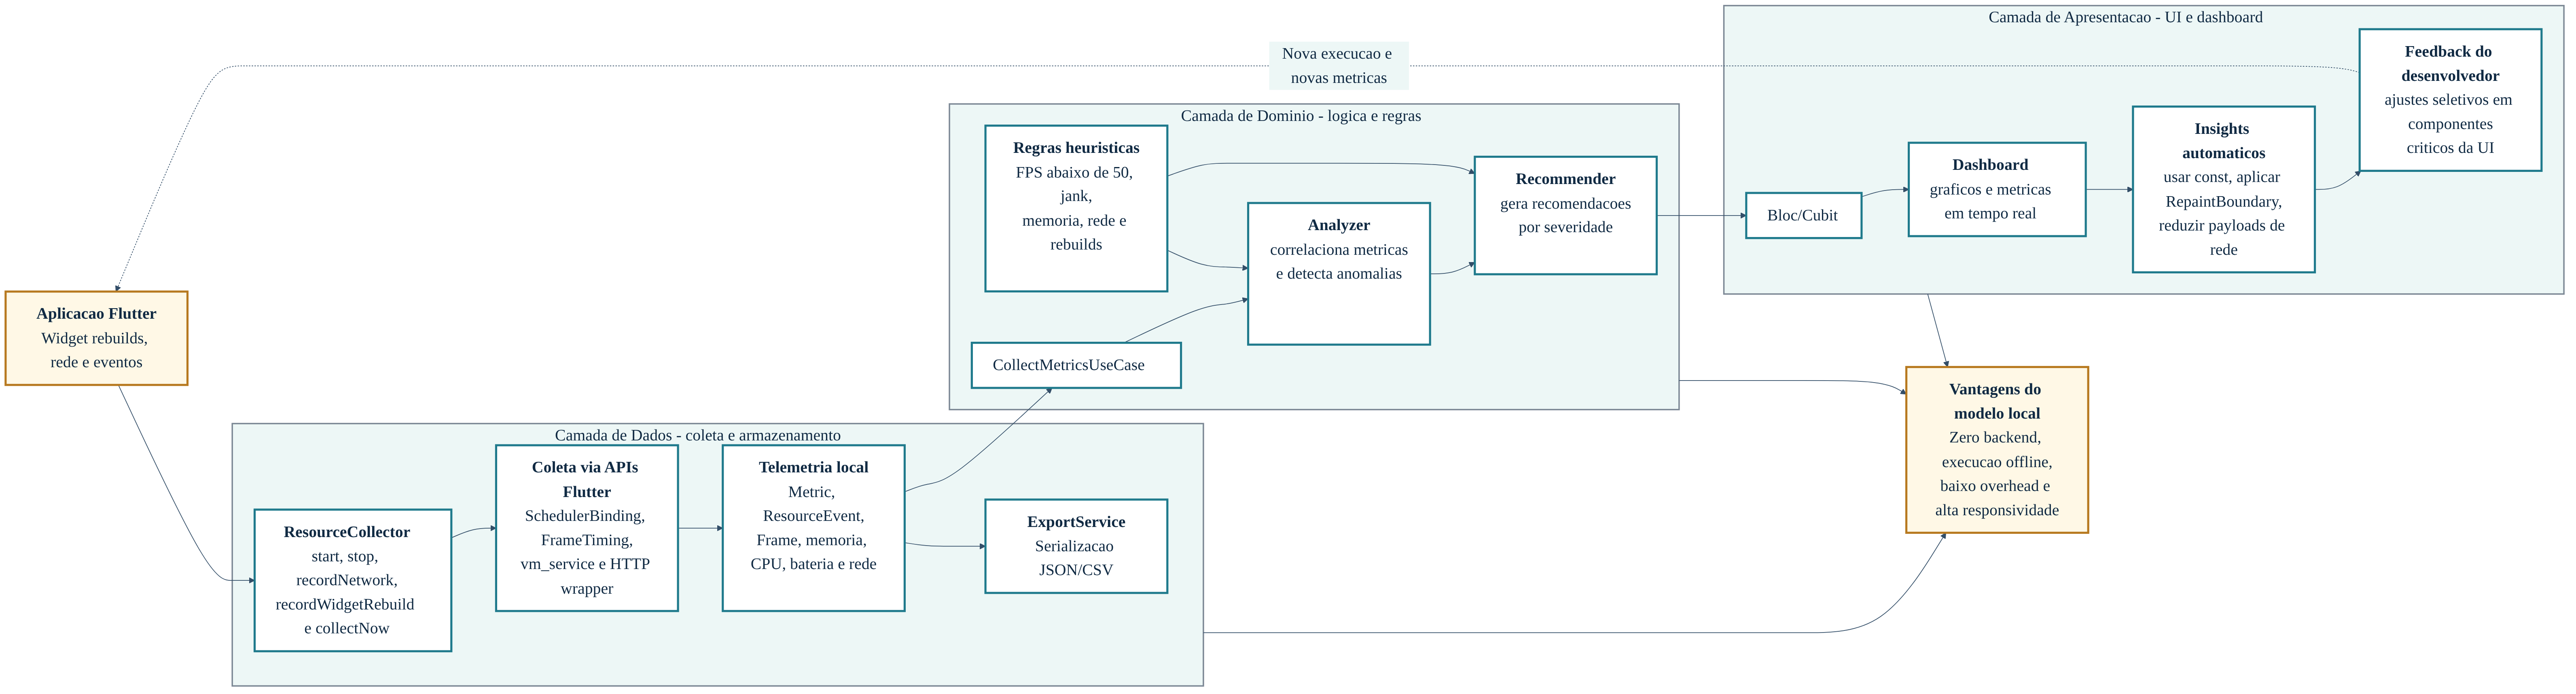
\includegraphics[width=\textwidth,height=0.66\textheight,keepaspectratio]{arquitetura_fluxo_collector.png}
  }{%
    \metric{\textwidth}{collectorTeal}{Data -> Domain -> Presentation}
  }
\end{columns}
\end{frame}

\begin{frame}{Dashboard integrado}
\chaptertag{Evidência visual do pacote}
\begin{columns}[T,onlytextwidth]
  \column{0.49\textwidth}
  \centering
  \IfFileExists{../images/figures/prototipoquandoestaok.jpeg}{%
    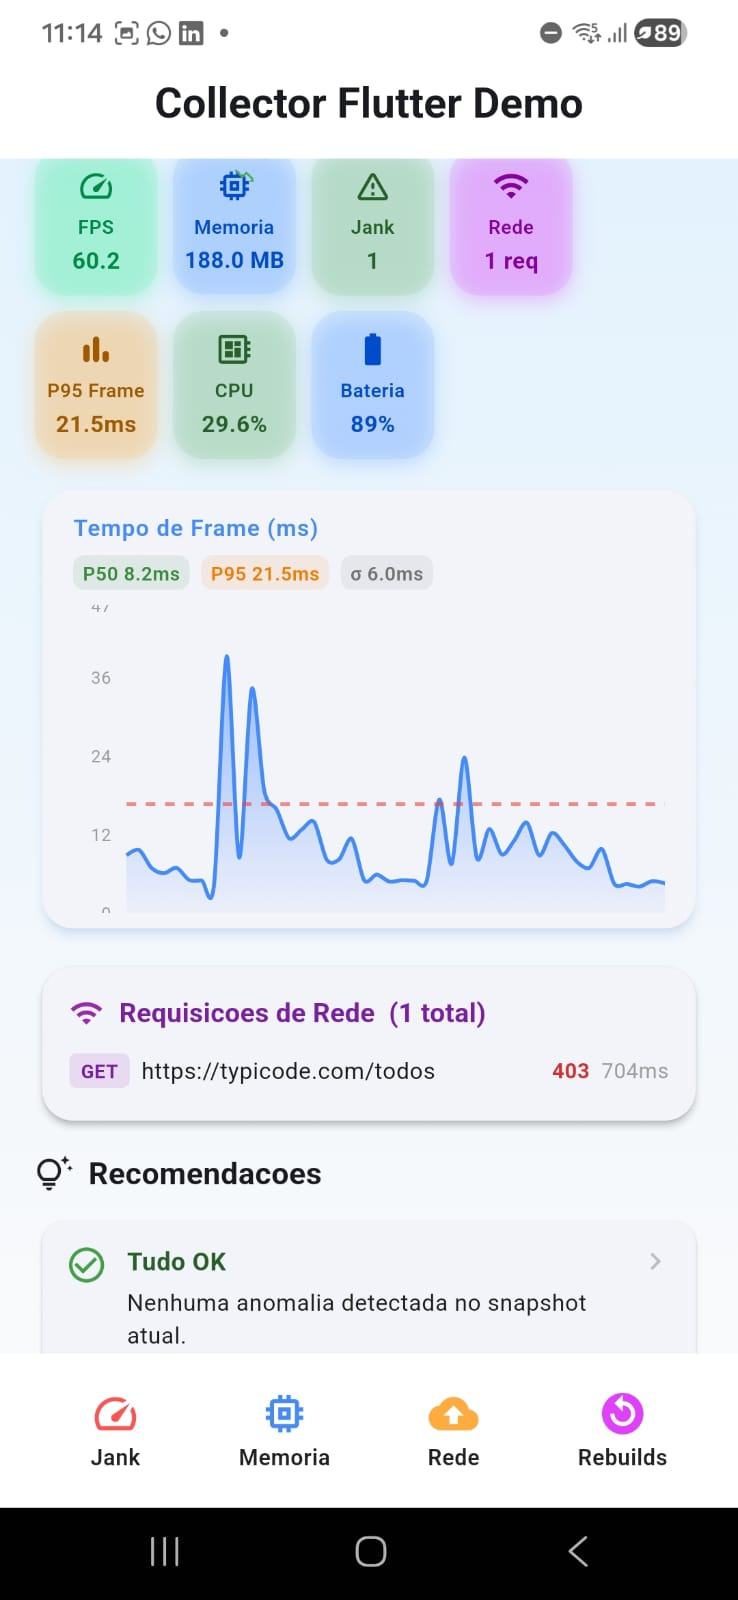
\includegraphics[height=0.69\textheight]{prototipoquandoestaok.jpeg}
  }{\metric{\textwidth}{collectorTeal}{Estado estável}}

  \small Estado estável
  \column{0.49\textwidth}
  \centering
  \IfFileExists{../images/figures/prototipoquandonaoestaok.jpeg}{%
    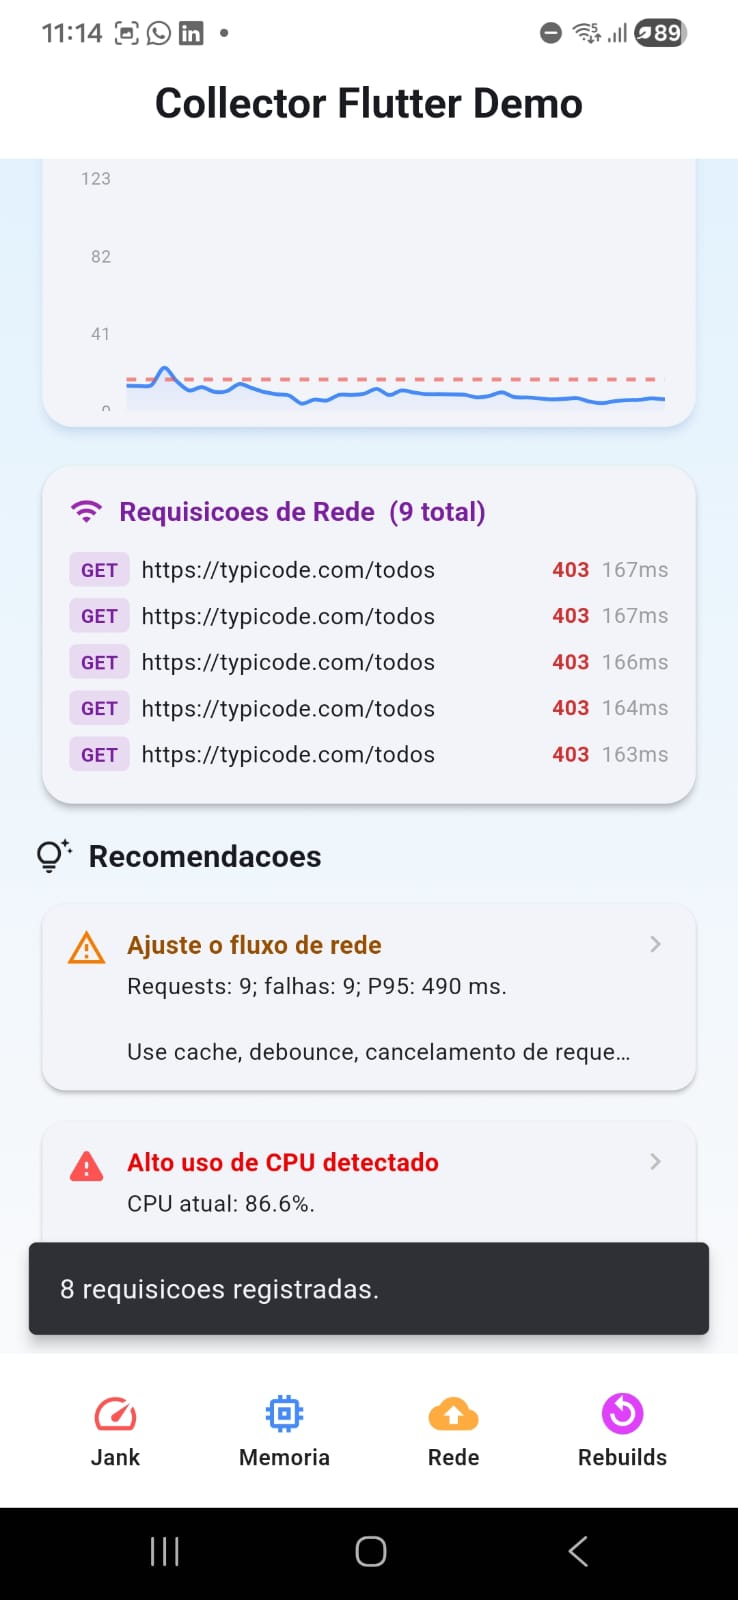
\includegraphics[height=0.69\textheight]{prototipoquandonaoestaok.jpeg}
  }{\metric{\textwidth}{collectorCoral}{Gargalos}}

  \small Gargalos detectados
\end{columns}
\end{frame}

\begin{frame}{Metodologia}
\chaptertag{Avaliação funcional}
\begin{columns}[T,onlytextwidth]
  \column{0.48\textwidth}
  \begin{itemize}
    \item Pesquisa aplicada: constrói uma solução prática.
    \item Ciclo iterativo: revisão, requisitos, implementação e validação.
    \item Execuções controladas no aplicativo de exemplo.
    \item Resultados tratados como evidência funcional, não estatística.
  \end{itemize}
  \column{0.48\textwidth}
  \centering
  \IfFileExists{../images/mermaid/outputs/metodologia_pesquisa.png}{%
    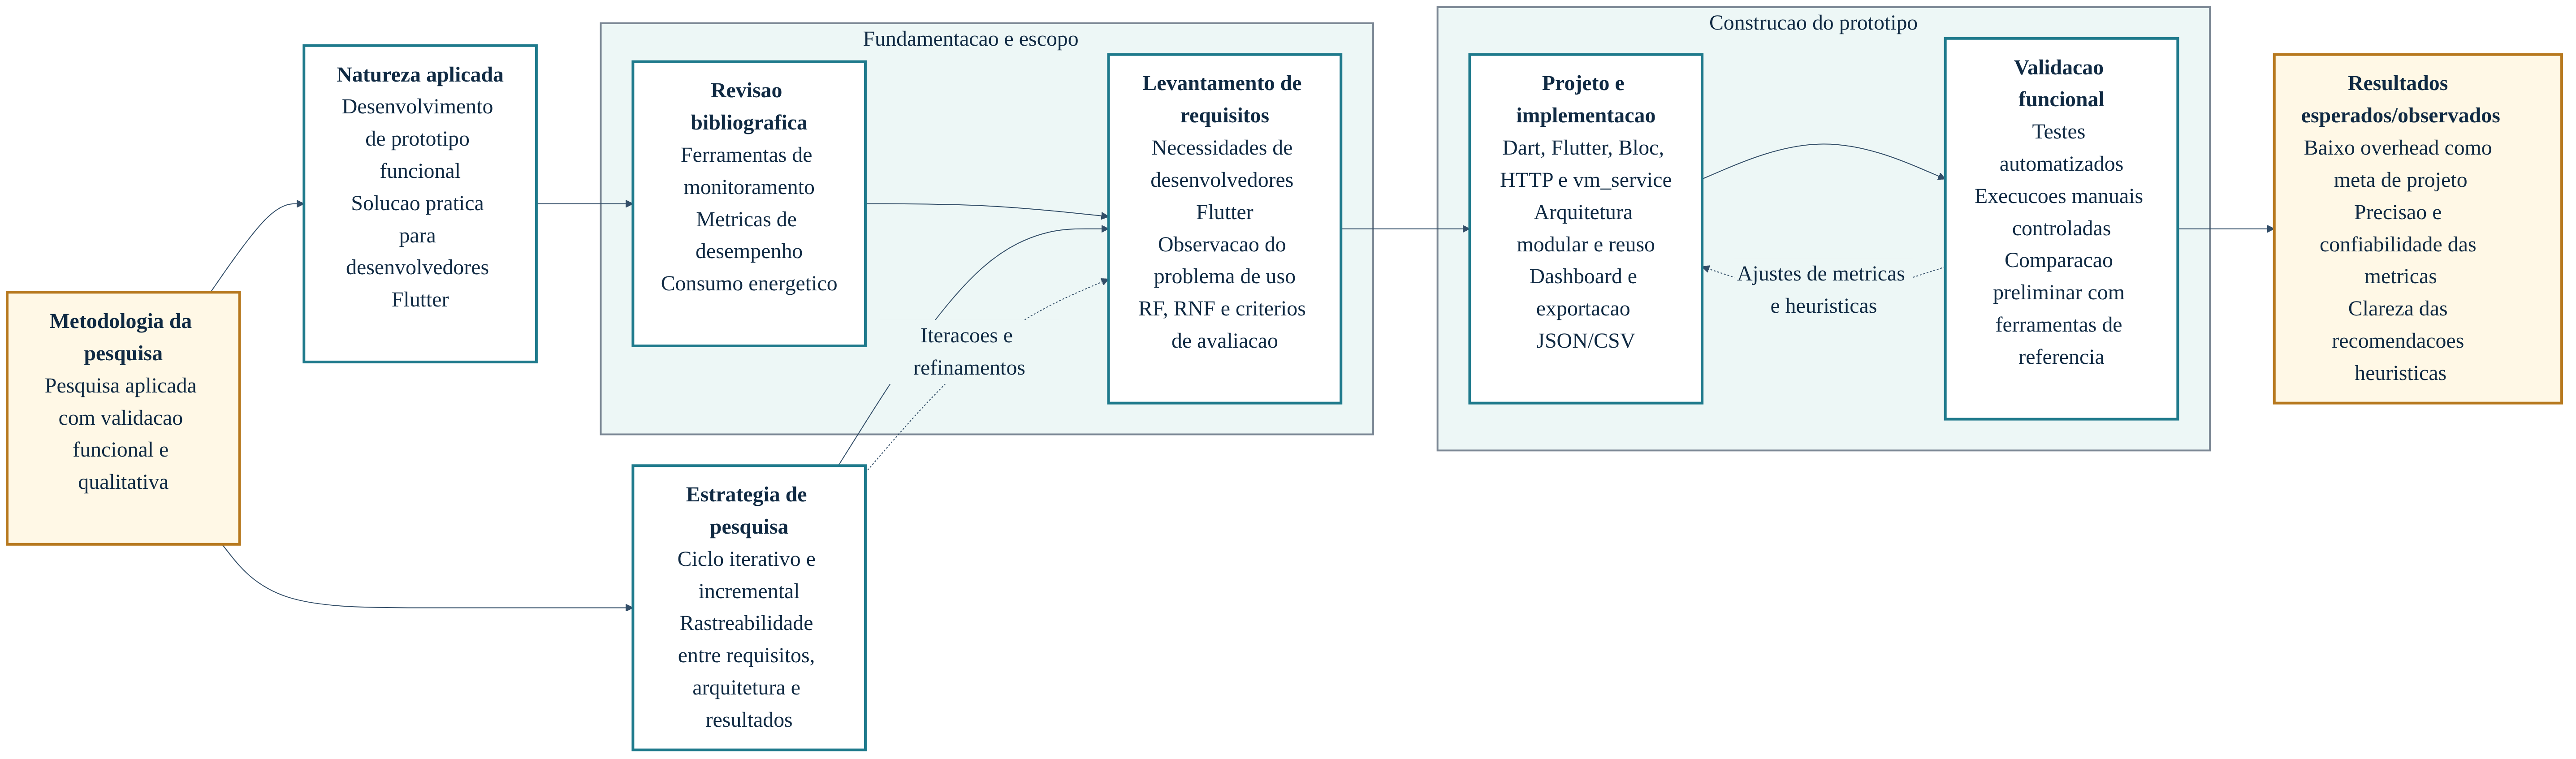
\includegraphics[width=\textwidth,height=0.58\textheight,keepaspectratio]{metodologia_pesquisa.png}
  }{%
    \metric{\textwidth}{collectorTeal}{Revisão -> pacote -> cenários -> análise}
  }
\end{columns}
\end{frame}

\begin{frame}{Cenários testados}
\chaptertag{Quatro cargas controladas}
\begin{columns}[T,onlytextwidth]
  \column{0.25\textwidth}
  \begin{accentbox}{1. Rebuilds}
    Reconstruções intensivas de interface.
  \end{accentbox}
  \column{0.25\textwidth}
  \begin{infobox}{2. Rede}
    Requisições HTTP simultâneas.
  \end{infobox}
  \column{0.25\textwidth}
  \begin{accentbox}{3. Memória}
    Alocação intensiva de objetos.
  \end{accentbox}
  \column{0.25\textwidth}
  \begin{infobox}{4. Combinado}
    Interface, rede, memória e CPU.
  \end{infobox}
\end{columns}
\vspace{3mm}
\begin{center}
\bfseries
Cada cenário provoca um sintoma esperado; o painel precisa tornar esse sintoma visível.
\end{center}
\end{frame}

\begin{frame}{Evidências dos cenários}
\chaptertag{Imagens geradas no projeto}
\begin{columns}[T,onlytextwidth]
  \column{0.25\textwidth}
  \centering
  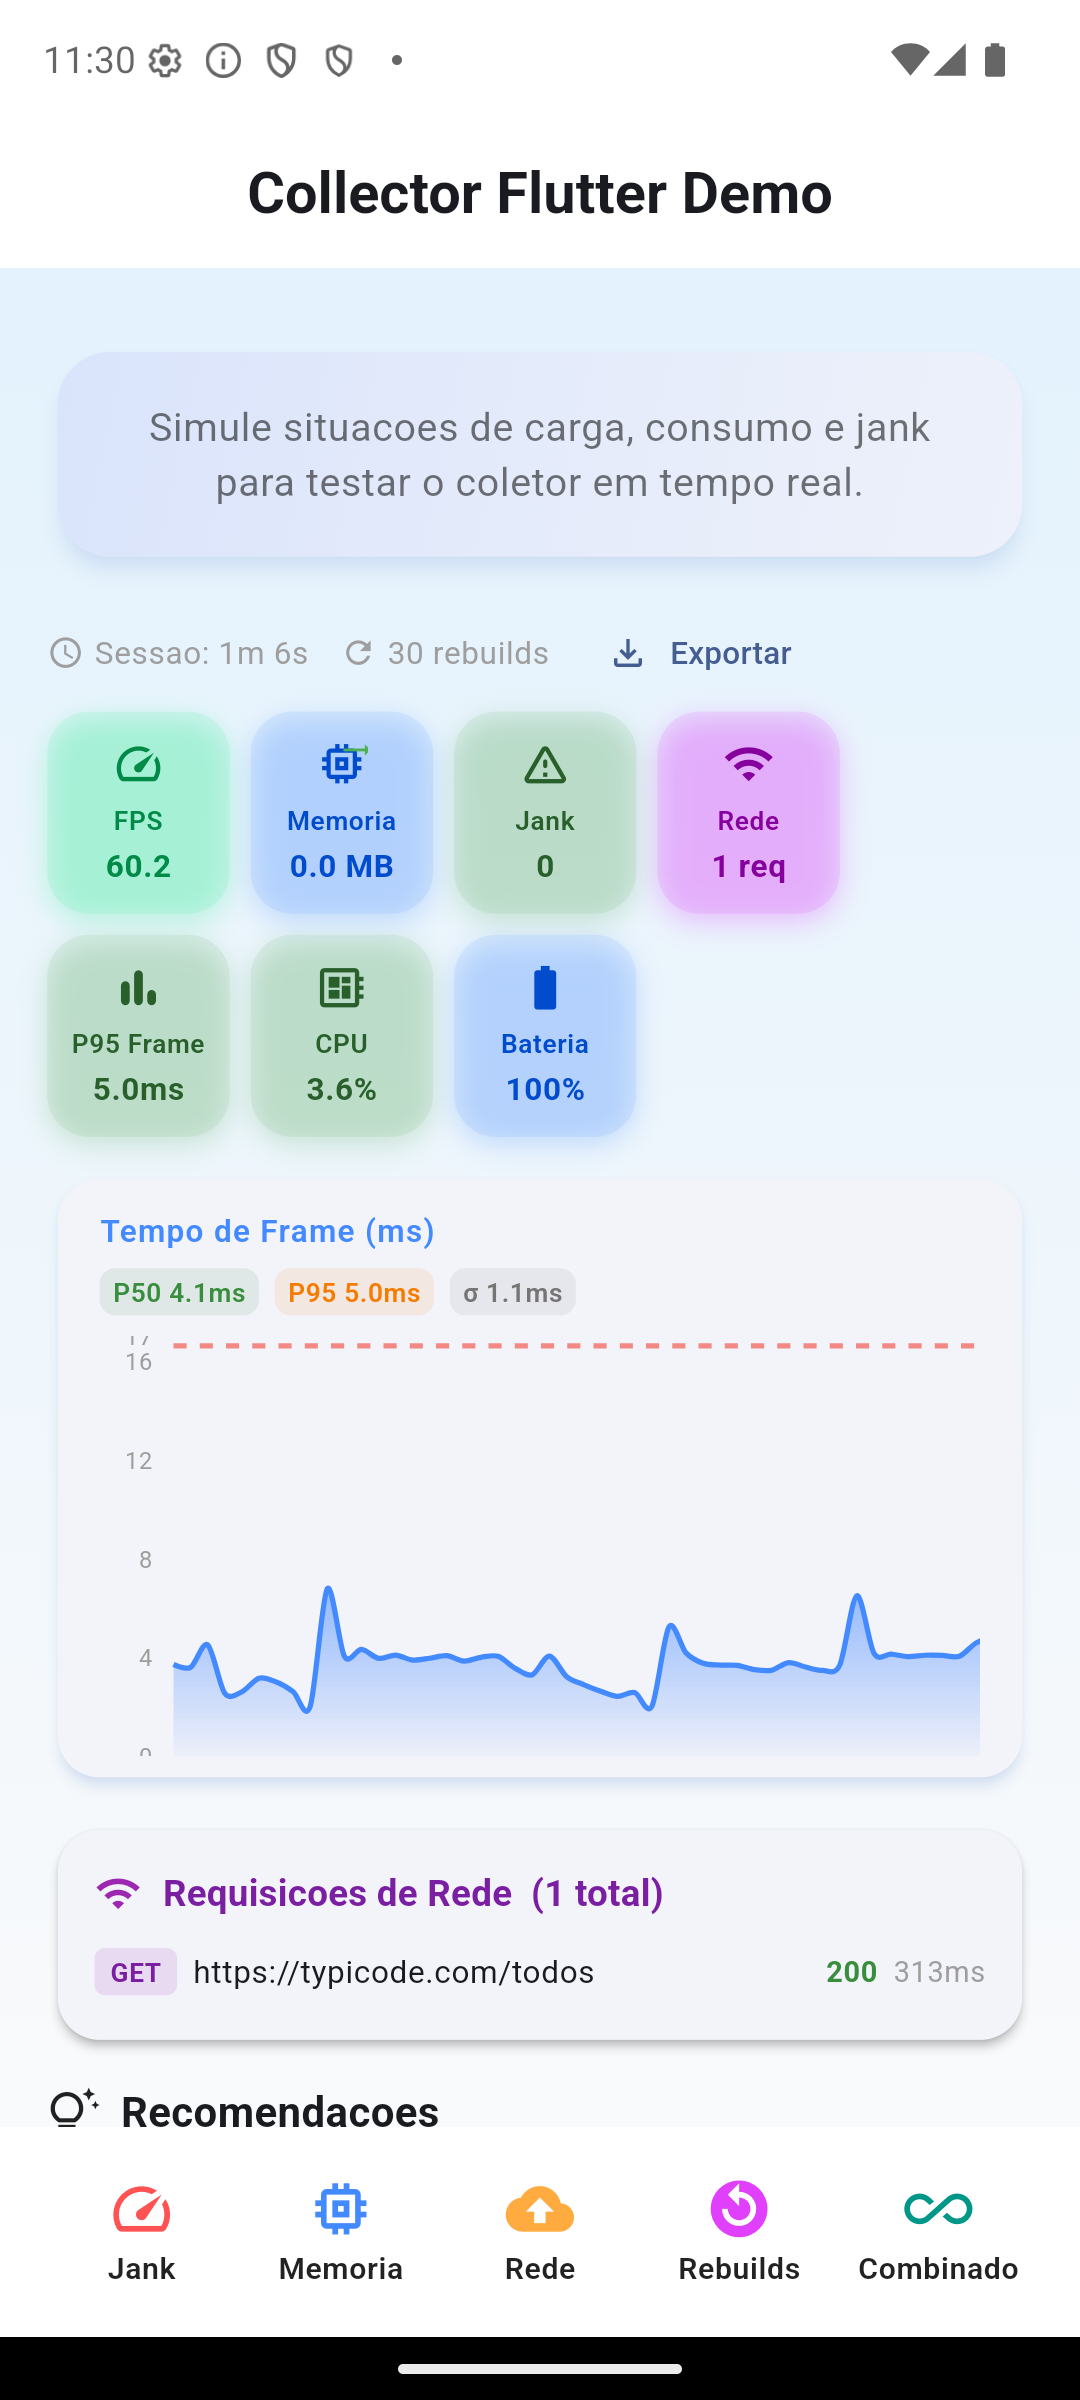
\includegraphics[height=0.60\textheight]{evidencia_cenario_rebuilds.png}

  \scriptsize Rebuilds
  \column{0.25\textwidth}
  \centering
  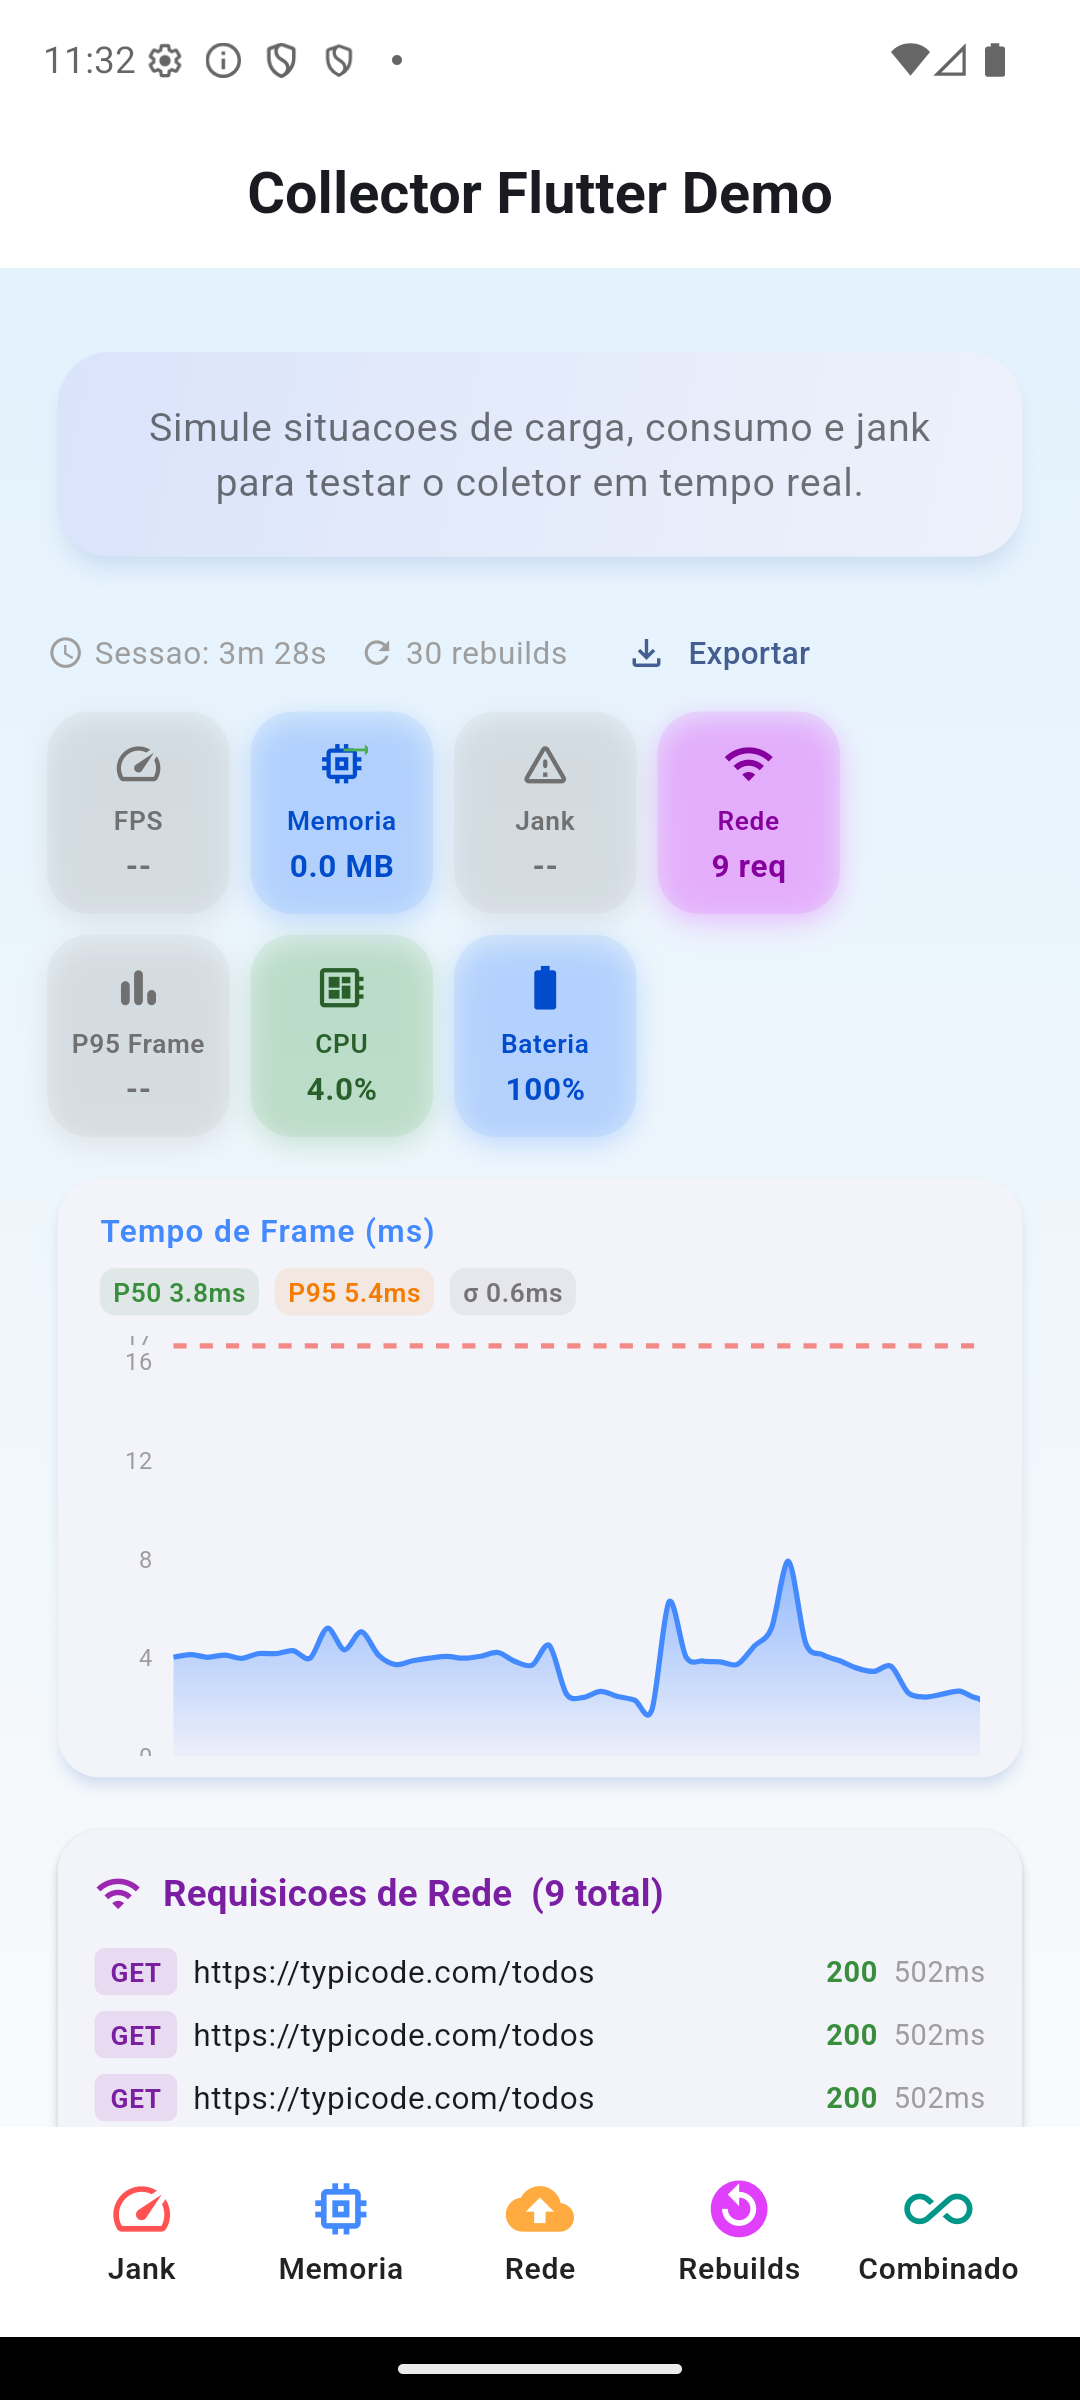
\includegraphics[height=0.60\textheight]{evidencia_cenario_rede.png}

  \scriptsize Rede
  \column{0.25\textwidth}
  \centering
  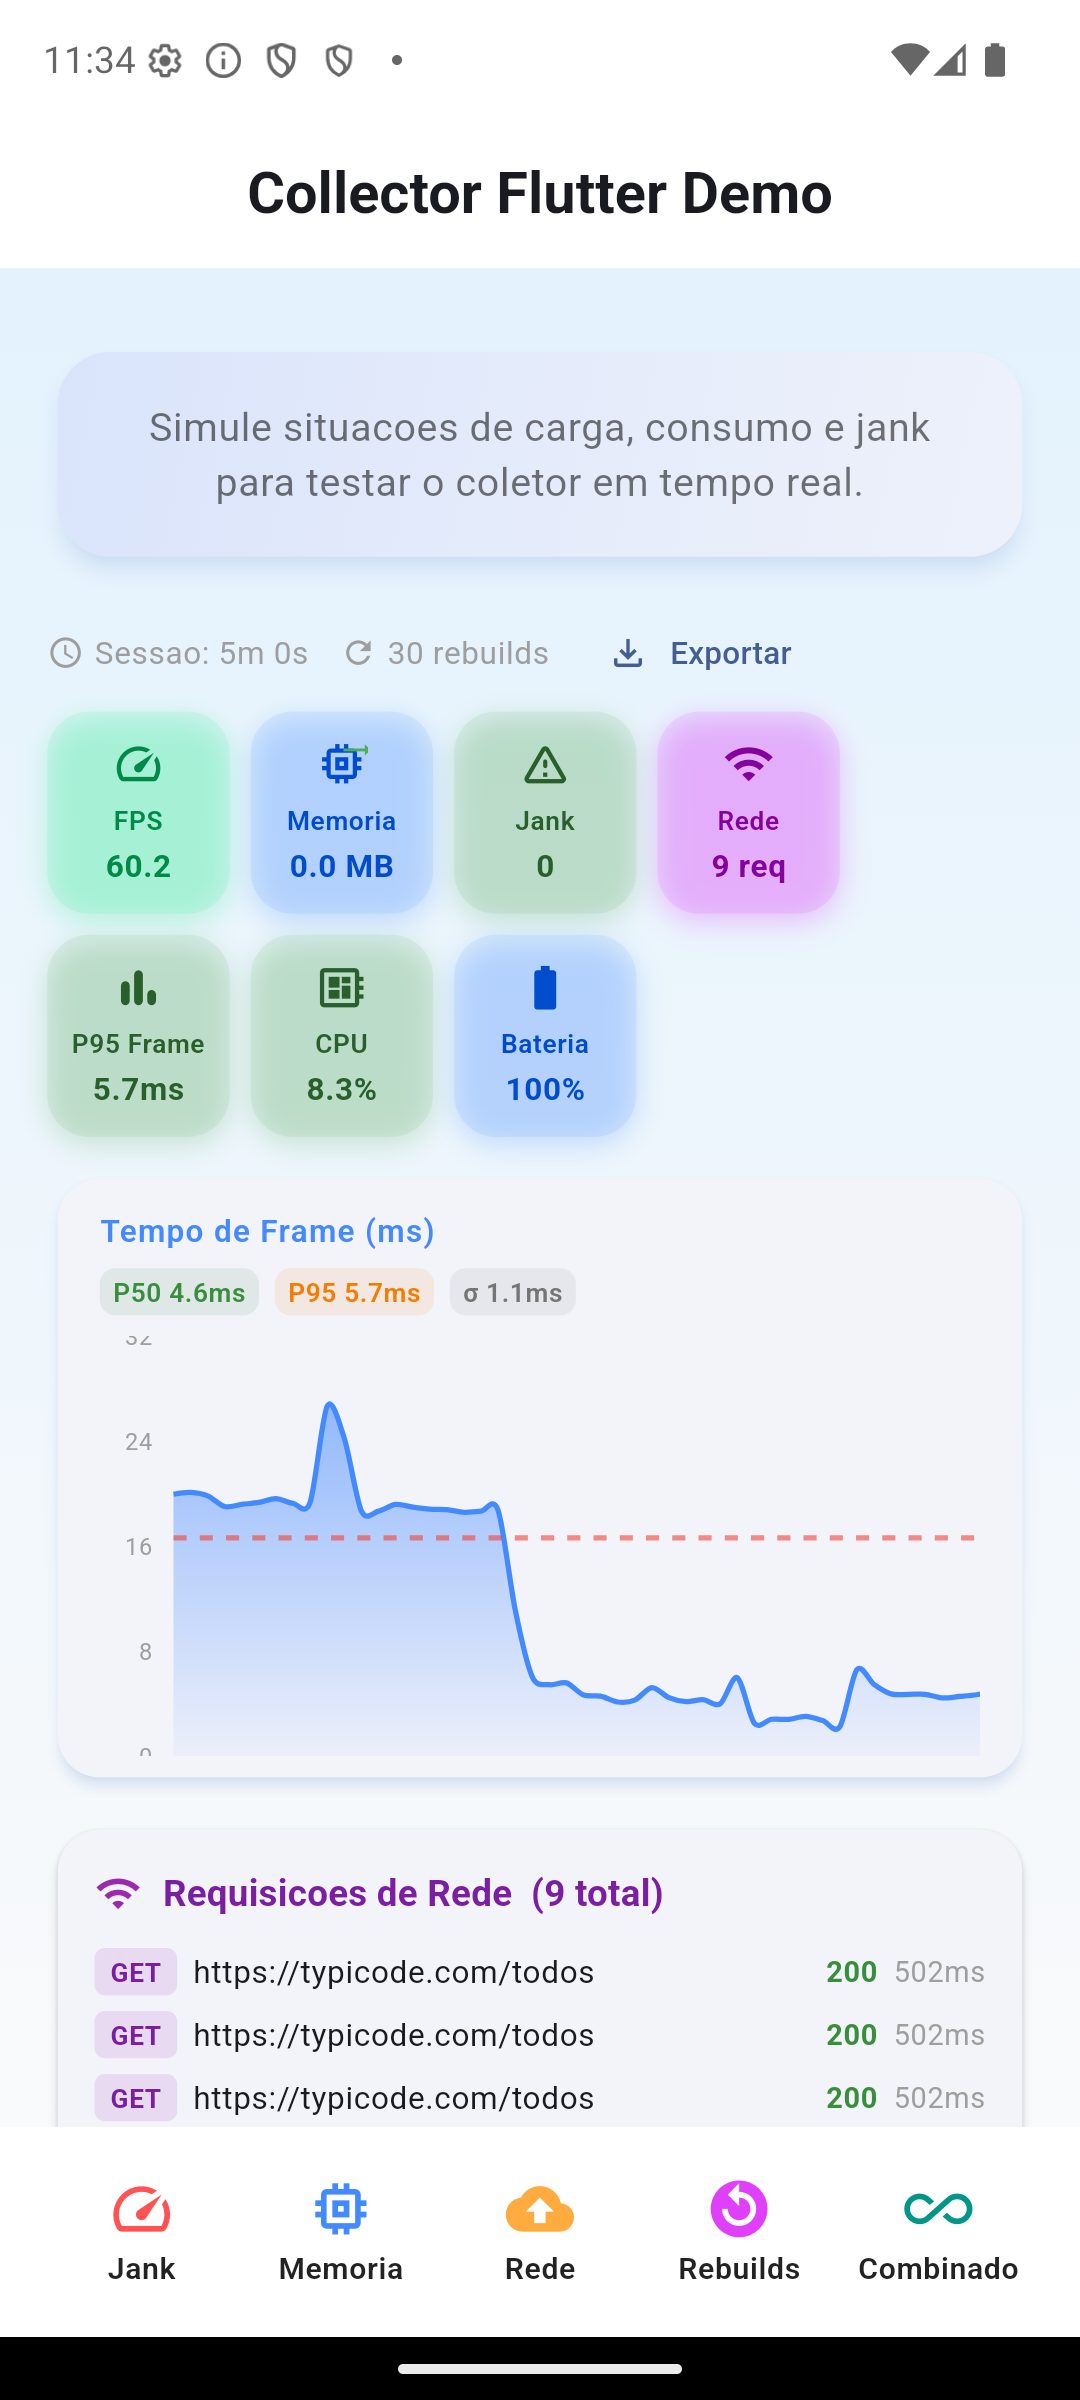
\includegraphics[height=0.60\textheight]{evidencia_cenario_memoria.png}

  \scriptsize Memória
  \column{0.25\textwidth}
  \centering
  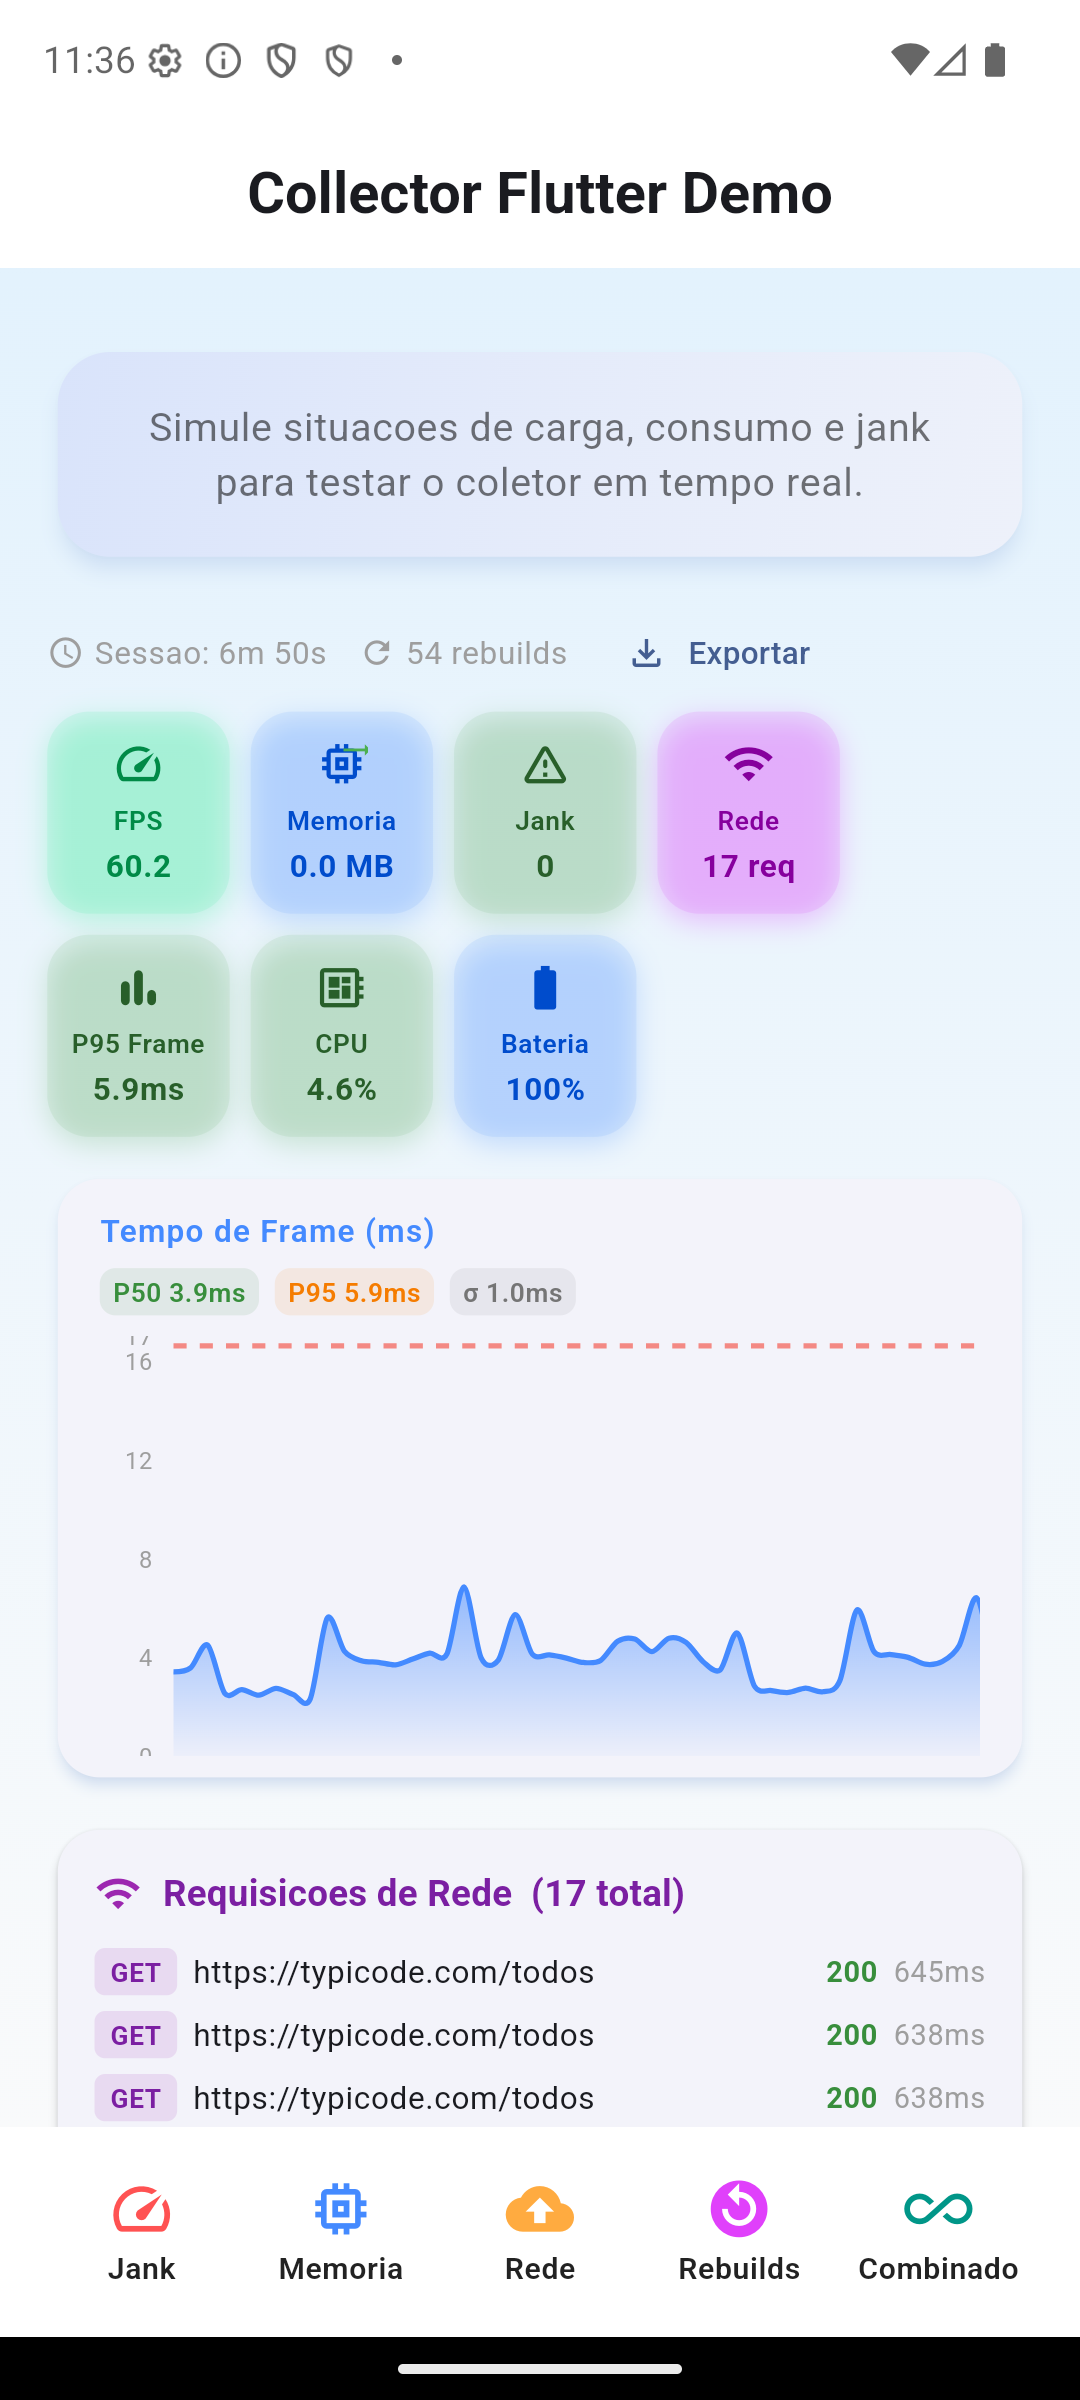
\includegraphics[height=0.60\textheight]{evidencia_cenario_combinado.png}

  \scriptsize Carga combinada
\end{columns}
\vspace{1mm}
\smallref{As capturas foram preservadas na monografia como Apêndice B, junto das leituras ADB.}
\end{frame}

\begin{frame}{Resultados observados}
\chaptertag{O que apareceu nos logs e no painel}
\footnotesize
\begin{tabularx}{\textwidth}{L{2.8cm}Y Y}
\toprule
\textbf{Cenário} & \textbf{Sinais registrados} & \textbf{Leitura para a defesa} \\
\midrule
Rebuilds & 30 \textit{rebuilds}, FPS 55{,}4, P95 20{,}4 ms e 2 frames longos. & O painel reagiu à carga de interface. \\
Rede & 9 requisições, FPS 42{,}9, P95 139{,}5 ms e 4 frames longos. & O interceptador registrou eventos e latências. \\
Memória & ADB: RSS 236.480 KB e PSS 222.232 KB. & Houve crescimento real, mas o snapshot do painel mostrou limitação de leitura. \\
Combinado & 17 requisições, 54 \textit{rebuilds}, FPS 44{,}6, P95 37{,}7 ms e CPU 75{,}3\%. & O sistema processou múltiplos sinais e priorizou alertas. \\
\bottomrule
\end{tabularx}
\vspace{1mm}
\smallref{Essa evidência mostra operacionalidade, não precisão estatística.}
\end{frame}

\begin{frame}{ADB, Profiler e limites}
\chaptertag{Transparência metodológica}
\begin{columns}[T,onlytextwidth]
  \column{0.5\textwidth}
  \begin{accentbox}{O que foi usado de fato}
    \begin{itemize}
      \item \texttt{adb shell dumpsys meminfo}
      \item \texttt{adb shell dumpsys gfxinfo}
      \item Logs \texttt{EVIDENCE} do aplicativo
      \item Capturas reais do emulador
    \end{itemize}
  \end{accentbox}
  \column{0.5\textwidth}
  \begin{infobox}{Como interpretar}
    Android Profiler e Perfetto ficaram como referências conceituais. Nesta avaliação, não houve série comparativa quantitativa nem cálculo formal de erro percentual.
  \end{infobox}
  \begin{accentbox}{Limitação importante}
    O \texttt{gfxinfo} confirmou a superfície Flutter, mas retornou contadores HWUI zerados nessa execução.
  \end{accentbox}
\end{columns}
\end{frame}

\begin{frame}{Testes automatizados}
\chaptertag{60 casos aprovados}
\begin{columns}[T,onlytextwidth]
  \column{0.46\textwidth}
  \metric{\textwidth}{collectorTeal}{60 testes}
  \begin{itemize}
    \item 24 em análise e estatísticas.
    \item 17 em CPU e bateria.
    \item 12 em recomendações.
    \item 7 em exportação.
  \end{itemize}
  \column{0.52\textwidth}
  \scriptsize
  \begin{tabular}{p{2.2cm}p{3.3cm}r}
  \toprule
  \textbf{Arquivo} & \textbf{Cobertura} & \textbf{Casos} \\
  \midrule
  Analyzer & \rule{2.8cm}{0.45em} & 24 \\
  CPU/bateria & \rule{2.0cm}{0.45em} & 17 \\
  Recommender & \rule{1.4cm}{0.45em} & 12 \\
  ExportService & \rule{0.8cm}{0.45em} & 7 \\
  \bottomrule
  \end{tabular}
  \vspace{3mm}

  \begin{infobox}{Papel dos testes}
    Eles verificam regras internas, serialização e fallbacks. Não substituem experimentos quantitativos em dispositivos reais.
  \end{infobox}
\end{columns}
\end{frame}

\begin{frame}{Limitações e trabalhos futuros}
\chaptertag{O que fica para evoluir}
\begin{columns}[T,onlytextwidth]
  \column{0.5\textwidth}
  \begin{infobox}{Limitações}
    \begin{itemize}
      \item Validação funcional, sem análise estatística.
      \item Foco principal em Android.
      \item Sem estudo formal de usabilidade.
      \item Comparação ADB apenas como apoio qualitativo.
    \end{itemize}
  \end{infobox}
  \column{0.5\textwidth}
  \begin{accentbox}{Trabalhos futuros}
    \begin{itemize}
      \item Rodadas quantitativas com múltiplos dispositivos.
      \item Séries comparáveis com Profiler, Perfetto e ADB.
      \item CPU e energia mais completas no iOS.
      \item Avaliação com desenvolvedores Flutter.
    \end{itemize}
  \end{accentbox}
\end{columns}
\end{frame}

\begin{frame}{Conclusão}
\chaptertag{Mensagem final}
\begin{itemize}
  \item O \collectorFlutter{} aproxima o primeiro diagnóstico de desempenho do fluxo real de desenvolvimento Flutter.
  \item A arquitetura em camadas permitiu evoluir o pacote com CPU, bateria, exportação e testes.
  \item Os quatro cenários controlados indicaram operacionalidade e recomendações compatíveis com os sintomas induzidos.
  \item A validação foi honesta sobre seus limites: funcional e qualitativa, com trabalhos futuros bem definidos.
\end{itemize}
\vspace{3mm}
\begin{accentbox}{Fechamento}
Performance não é apenas fazer o app rodar mais rápido; é fazer o app respeitar melhor o dispositivo, a bateria e a pessoa que o usa.
\end{accentbox}
\end{frame}

\begin{frame}[plain]
\centering
\vspace{15mm}
{\Huge\bfseries Perguntas?}

\vspace{7mm}
{\Large \collectorFlutter{}}

\vspace{7mm}
\IfFileExists{../images/figures/logo2.png}{
\includegraphics[height=0.7cm]{logo2.png}}{}
\hspace{10mm}
\IfFileExists{../images/figures/logo1.jpeg}{
\includegraphics[height=1cm]{logo1.jpeg}}{}

\vfill
\small Beatriz Vocurca Frade \quad | \quad Engenharia de Sistemas -- UFMG
\end{frame}

\end{document}
